% Introduction
% historical timeline
% reference some explanatory pictures
% introduce some notation
% main takeaways the mathematical elements are simple but notation is
%a limitation.
\part{Introduction} % Main chapter title
\label{Chapter1} % For referencing the chapter elsewhere, use \ref{Chapter1} 

% \begin{frame}[fragile]
% \frametitle{Neural Network}

% \scalebox{.9}{
% \begin{frame}[fragile]
% \frametitle{Neural Network}

% \scalebox{.9}{
% }
% \end{frame}

%%%%%%%%%%%%%%%%%%%%%%%%%%%%%%%%%%%%%%%%%(1)
\begin{frame}
  \frametitle{Goals}
  \begin{itemize}
      % \item<1-> Describe brief history of machine-learning. 
      \item<1-> Understand (mathematically) what Artificial Neural
        Networks (ANNs) are and how they are being used. 
      \item<2-> Define a geometric approach to interpreting neural
        network classifiers. 
      \item<3-> Connect geometric approach with concept of 
        robustness. 
      \item<4-> Define a kernel based representation which allows application
        of kernel based tools to ANNs
      \item<5-> Leverage our kernel based representation and these
        tools to get some useful results!
      \item<6-> Lay out further work which will connect representation
        approach to the geometric properties observed earlier. 
  \end{itemize}
\end{frame}

% transition from task specific models to foundation models --
% Models are starting to have a "general" geometric understanding of
% the data. 
\section{Background}

\begin{frame}
  \frametitle{History : Beginnings in Theory of Cognition}
  \begin{itemize}
     \item<1->  The mechanics of cognition are described in the context of
      computation by ~\citet{mcculloch1943logical}. 
      \item<2-> The perceptron $f(x) = A(w \cdot x + b)$, the
        most granular element of a neural network, is proposed by
        ~\citet{rosenblatt1958perceptron}. 
      \item<3->  Perceptrons are assembled into multilevel (deep)
        networks ($A_n \circ f_n \circ
        \cdots \circ f_3 \circ A_2 \circ f_2 \circ
        A_1 \cdots f_1$) by ~\citet{ivakhnenko1965cybernetic}
      \item<5->  ~\citet{minsky1969perceptrons} present a proof that
        basic perceptrons could not encode exclusive-or. 
      \item<6->  Neural Networks become disassociated from Cognitive
        Science and Computational Limitations curtail industrial
        applications. 
      \item<7-> Interest in Neural Networks wanes. 
  \end{itemize}
\end{frame}

\begin{frame}
  \frametitle{History : Revolution}
  \begin{itemize}
      \item<1-> ~\citet{linnainmaa1970representation} proposes
        a computation for gradients of large-scale multi-parameter
 models in his masters thesis. Back-Propagation is born!
      \item<2->  A Harvard student,  ~\citep{werbos1974beyond},
        applies this technique to ANNs. 
      \item<3->  ~\citet{mcclelland1986parallel} propose distributed
        processing in the context of cognition allowing tree-like
        computations to be processed in separate computing threads. 
      \item<4-> Finally, these pieces are brought together by
        ~\citet{lecun1989backpropagation}. 
      \item<5->  ~\citep{lecun1995convolutional} invent convolutional
        neural networks which are more capable and scale more
        cheaply.
        \item <6-> This completed tools is applied to the
        lucrative task of handwriting recognition
        ~\citep{lecun1998gradient} and the commercial viability of
        ANNs is established. 

  \end{itemize}
\end{frame}

\begin{frame}
  \frametitle{History : Explosion}
  \begin{itemize}
     \item<1-> Neural Networks' industrial success fuels a new wave of
       serious research and development including the now famous
       PyTorch ~\citep{Collobert2002TorchAM} 
       
     \item<2-> Geoffrey Hinton is among the first to comprehensively understand
       how to scale ``deep'' learning models
       ~\citep{hinton2006reducing, hinton2006fast} along with Samy
       Bengio ~\citep{bengio2009learning}. 

       % \item<3-> Recurrent networks, applying  earlier work on
       %   Long-Short-Term-Memory (LSTM) networks
       %   ~\citep{hochreiter1997long} to overcome vanishing gradients, are implemented
       %   ~\citep{mikolov2010recurrent}. 

       \item<3-> Recurrent ANNs are applied to natural
language processing ~\citep{collobert2011natural}
       \item<4-> ~\citet{szegedy2013} discover easily scalable
         adversarial attacks against neural networks!

      \item<5-> Networks trained on Google's ImageNet database (>14M
        images, >20K categories) outperform humans on classification
        tasks \citep{SCHMIDHUBER201585}
      \visible<4>{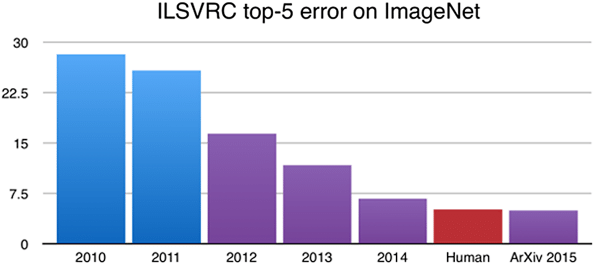
\includegraphics[width=7cm]{imnet_progress.png}}
  \end{itemize}
\end{frame}


\subsection{Structure}
% In this subsection we give a mathematical description of artificial neural networks. 

% %TODO: change this definition to something very vague and general -- use wikipedia 
% \begin{definition}{A \textbf{Neuron} is  }
%    a nonlinear operator that takes input in $\R^n$ to $\R$, historically designed to emulate the activation characteristics of an organic neuron.
%    \end{definition}

% \begin{frame}
%   \frametitle{Definitions : ANN}
% \begin{definition}{A \textbf{Neuron} is  } a nonlinear operator that
%   takes input in $\R^n$ to $\R$, historically designed to emulate the
%   activation characteristics of an organic neuron. A collection of
%   neurons that are connected via a (usually directed) graph structure
%   are known as an \emph{Artificial Neural Network (ANN)}.
% \end{definition}


% \end{frame}
\begin{frame}
  \frametitle{Definitions : Building Blocks}

The fundamental building blocks of most ANNs are artificial neurons which we will refer to as \emph{perceptrons}.

\begin{definition}{A \textbf{Perceptron} is  }
\label{perceptron}
a function $P_{\vec w}: \R^n \to \R$ which has \emph{weights} $\vec
w \in \R^n$ corresponding with each element of an input vector $\vec
x\in \R^n$ and a bias $b \in \R$:
\[P_{\vec w}(\vec x) = f(\left(\ip{\vec w,\vec x} + b\right)\]
\[P_{\vec w}(\vec x) = f\left(b + \sum_{i = 1}^n w_i x_i\right)\]
where $f: \R \to \R$ is continuous. The function $f$ is called the \textbf{activation function} for $P$. 
\end{definition}

\end{frame}

\begin{frame}
  \frametitle{Definitions : Perceptron}
  Perceptrons have a few notable properties
  \begin{itemize}
  \item $w \cdot x + b$ is linear.
    \item The activation function $f$ must contain all non-linearity
      needed for universal function approximation.
      \item In order to approximate arbitrary nonlinear functions, $f$ must
        not be linear ~\citep{attali1997approximations}.
        \item Arbitrarily many perceptrons can be connected in a
          tree-structure.
\end{itemize}
\end{frame}
      

\begin{frame}
 \frametitle{Definitions : ReLU}
\begin{definition}{The Rectified Linear Unit (ReLU) function is}
\label{relu}
   \[\relu(x) = \begin{cases} 0, & x \leq 0;\\
       x, & x > 0,\end{cases}\]
 \end{definition}

\begin{itemize}
    \item ~\citet{glorot2011deep} showed that
      Rectified Linear Units (ReLU) can out-perform smoother
      activation functions e.g. sigmoids.
    \item ReLU Networks even converge faster according to
      ~\citet{nair_rectified_nodate}!
    \item  ~\citet{petersen2018optimal} demonstrated that this single
      nonlinearity of this activation function
at $x = 0$ is sufficient to guarantee existence of $\epsilon$ approximation of smooth functions
\end{itemize}
\end{frame}





% In general ANNs 
% must not be cyclic and, for convenience, are often arranged into
% independent layers. An early roadblock for neural networks was a proof
% by ~\citet{minsky1969perceptrons} that single layers of perceptrons
% could not encode exclusive-or. ~\citet{kak1993training} demonstrated
% that depth, the number of layers in a neural network, is a key factor in its ability to approximate complicated functions including exclusive-or . For this reason, modern ANNs are usually composed of many layers (3-100). The most common instance of a neural network model is a fully connected \emph{feed forward (FF)} configuration. In this configuration data enters as an input layer which is fed into each of the nodes in the first layer of neurons. Output of the first layer is fed into each of the nodes in the second layer, and so on until the output of the final layer is fed into an output filter which generates the final result of the neural network. 



\begin{frame}
  \frametitle{Example : Fully Connected Feed Forward Network}
% In this example of a FF network, an input vector in $\R^7$ is mapped to a
% an output in $\R^3$ which is fed into a classifier. Each blue circle
% represents a perceptron with the ReLU activation function. 
\centering
\scalebox{.9}{
\begin{tikzpicture}[shorten >=1pt,->,draw=black!50, node distance=\layersep]
    \tikzstyle{every pin edge}=[<-,shorten <=1pt]
    \tikzstyle{neuron}=[circle,fill=black!25,minimum size=9pt,inner sep=0pt]
    \tikzstyle{input neuron}=[neuron, fill=green!50];
    \tikzstyle{output neuron}=[neuron, fill=red!50];
    \tikzstyle{hidden neuron}=[neuron, fill=blue!50];
    \tikzstyle{annot} = [text width=4em, text centered]

    % Draw the input layer nodes
    \foreach \name / \y in {1,...,7}
    % This is the same as writing \foreach \name / \y in {1/1,2/2,3/3,4/4}
        \node[input neuron] (I-\name) at (0,-\y) {};
%pin=left:Input \#\y
    % Draw the hidden layer nodes
    \foreach \name / \y in {1,...,6}
        \path[yshift=-0.5cm]
            node[hidden neuron] (H-\name) at (\layersep,-\y cm) {};

    \foreach \name / \y in {1,...,4}
        \path[yshift=-1.5cm,xshift=2.0cm]
            node[hidden neuron] (HH-\name) at (\layersep,-\y cm) {};

    \foreach \name / \y in {1,...,3}
        \path[yshift=-2cm,xshift=4.0cm]
            node[output neuron] (O-\name) at (\layersep,-\y cm) {};

    % Draw the output layer node
%   \foreach \name / \y in {1,...,3}
%        \path[yshift=-1.5cm,xshift=4.0cm]
%            \node[output neuron] (O-\name) at (\layersep,-\y cm) {};


    % Connect every node in the input layer with every node in the
    % hidden layer.
    \foreach \source in {1,...,7}
        \foreach \dest in {1,...,6}
            \path (I-\source) edge (H-\dest);

    \foreach \source in {1,...,6}
        \foreach \dest in {1,...,4}
            \path (H-\source) edge (HH-\dest);

    % Connect every node in the hidden layer with the output layer
    \foreach \source in {1,...,4}
        \foreach \dest in {1,...,3}
            \path (HH-\source) edge (O-\dest);

    % Annotate the layers
  \node [rectangle, draw, minimum height=6.2cm, text width=.8cm, text
  centered, left =.8cm of I-4] (mm) {Data};

    \foreach \source in {1,...,7}
        \path [line] (mm.east|-I-\source) -- (I-\source);

    \node[annot,above of=H-1, node distance=2cm] (hl) {Layer 1};
    \node[annot,left of=hl] {Input };
    \node[annot,right of=hl] (h3) {Layer 2} ;
    \node[annot,right of=h3] {Output Layer};
  \node [rectangle, draw, minimum height=5cm, text width=1.6cm, text
  centered, right =6.8cm of I-4] (mc) {Classifier};
    \foreach \source in {1,...,3}
        \path [line] (O-\source) -- (mc.west|-O-\source);


\end{tikzpicture}
}
\end{frame}


% The output of this ANN is fed into a classifier. To complete this
% example, we can define the most common classifier, Softmax:

\begin{frame}
  \frametitle{Definition : Softmax Classifier}
\begin{definition}{Softmax (or the normalized exponential) is the function given by}
\[s : \R^n \to [0,1]^n\]
\[s_j(\vec x) = \frac{e^{x_j}}{\sum_{k = 1}^n e^{x_k}}\]
\end{definition}

\begin{definition}{We can define a classifier which picks the class corresponding with the largest output element from Softmax: }
\[\text{(Output Classification)  }   c_s(\vec x) = \text{argmax}_{i} s_i(\vec{x})\]
\end{definition}
\end{frame}

% % It is important that the classifier admit a directed error function
% During training, the output $y \in \R^n$ from a network can thus be
% compressed using softmax into $[0,1]^n$ as a surrogate for probability
% for each possible class or directly into the classes which we can
% represent as the simplex for the vertices of $[0,1]^n$
% \citep{Bishop:2006:PRM:1162264}. 

% \subsubsection{Convolutional Neural Networks (CNNs)}\label{cnn}

\begin{frame}
  \frametitle{Example : Other Network Structures}
  \begin{itemize}
    \item \textbf{Convolutional Neural Networks} (CNNs) arrange nodes
      spatially and convolve kernels across this spatially producing
      output with multiple channels (corresponding with each
      individual kernel used) and preserving spatial adjacency.
    \item \textbf{Recurrent Neural Networks} (RNNs) admit prior
      network activations as inputs during computation allowing 
      limited ``memory'' while working on time-varying data.
\end{itemize}
\end{frame}
      

\begin{frame}
  \frametitle{Training ANNs}
  \begin{enumerate}
  \item Pick a Training Set
  \item Pick a loss function
     One commonly used loss function for classification is known as Cross-Entropy Loss:
 \begin{definition}{The Cross-Entropy Loss comparing two possible outputs is}
 $L(y,\hat y) = -\sum_i y_i \log \hat y_i$.
 \end{definition}
(Other commonly used loss functions include $L^1$ loss (also referred
to as Mean Absolute Error (MAE)), $L^2$ loss (often referred to as
Mean-Squared-Error (MSE)), and Hinge Loss (also known as SVM loss). )
\item Pick a first-order optimization scheme (ODE solver).
  \end{enumerate}
\end{frame}



\begin{frame}
  \frametitle{Training : Optimization}
  
 To set up the optimization, the loss for each training example must be aggregated. Generally, ANN training is conducted via Empirical Risk Minimization where Empirical Risk is defined for a given loss function $L$ as follows:
 \begin{definition}{Given a loss function $L$, the Empirical Risk over a training dataset $(X,Y)$ of size $N$ is }
 \[R_{\text{emp}}(P_{\vec w}(x) = \dfrac{1}{N} \sum_{(x,y) \in (X,Y)} L(P_{\vec w}(x)), y).\]
 \end{definition}
 We seek parameters $\vec w$ which will minimize $R_{\text{emp}}(P_{w}(x))$. This will be done with gradient-based optimization. 
\end{frame}

\begin{frame}
\frametitle{Computation of Gradient via Backpropagation}

\scalebox{.9}{
\begin{tikzpicture}[shorten >=1pt,->,draw=black!50, node distance=\layersep]

\node[circle, minimum size=19pt, fill=black!25, inner sep=0pt] (n11) at (0,2) {$a^1_1$};
\node[circle, minimum size=19pt, fill=black!25, inner sep=0pt] (n12) at (0,0) {$a^1_2$};
\node[circle, minimum size=19pt, fill=black!25, inner sep=0pt] (n21) at (4,2) {$a^2_1$};
\node[circle, minimum size=19pt, fill=black!25, inner sep=0pt] (n22) at (4,0) {$a^2_2$};
\node[circle, minimum size=19pt, fill=black!25, inner sep=0pt] (n31) at (8,2) {$a^3_1$};
\node[circle, minimum size=19pt, fill=black!25, inner sep=0pt] (n32) at (8,0) {$a^3_2$};

\node (av1) at (0,2.9) {$\Bar{a}^1$};
\node (av2) at (4,2.9) {$\Bar{a}^2$};
\node (av3) at (8,2.9) {$\Bar{a}^3$};

\node (ai1) at (0,3.9) {Index: $i$};
\node (ai2) at (4,3.9) {Index: $\alpha$};
\node (ai3) at (8,3.9) {Index: $\lambda$};

\node (w2) at (2.6,2.9) {$W^2$};
\node (w3) at (6.6,2.9) {$W^3$};


\draw[- triangle 45] (n11)  -- node[rotate=0,shift={(0.3,0.3)}] {$w^2_{1,1}$} (n21);
\draw[- triangle 45] (n11)  -- node[rotate=0,shift={(0.6,0.65)}] {$w^2_{1,2}$} (n22);
\draw[- triangle 45] (n12)  -- node[rotate=0,shift={(0.3,-0.65)}] {$w^2_{2,1}$} (n21);
\draw[- triangle 45] (n12)  -- node[rotate=0,shift={(0.6,-0.3)}] {$w^2_{2,2}$} (n22);

\draw[- triangle 45] (n21)  -- node[rotate=0,shift={(0.3,0.3)}]  {$w^3_{1,1}$} (n31);
\draw[- triangle 45] (n21)  -- node[rotate=0,shift={(0.6,0.65)}] {$w^3_{1,2}$} (n32);
\draw[- triangle 45] (n22)  -- node[rotate=0,shift={(0.3,-0.65)}]  {$w^3_{2,1}$} (n31);
\draw[- triangle 45] (n22)  -- node[rotate=0,shift={(0.6,-0.3)}]  {$w^3_{2,2}$} (n32);
\end{tikzpicture}
}
Where $x^{\text{[layer]}}_{\text{[node in layer], [node in previous
    layer]}}$

Recursively, we will define
\begin{equation}
    a^n_\lambda = A^n(\sum_\alpha w^n_{\alpha, \lambda} a^{n-1}_\alpha)
\end{equation}
\end{frame}

\begin{frame}
  \frametitle{Computation of Gradient via Backpropagation}
Given a loss function $L = \sum_{i} \ell_i(a^n_i)$ where each $\ell_i$ is a loss function on the $i^{\text{th}}$ element of the output, we wish to compute the derivatives $\dfrac{\partial L}{\partial_{w^l_{i,j}}}$ for every $l, i,$ and $j$ which compose the gradient $\nabla L$. Using the diagram above, we can compute this directly for each weight using chain rule:
\begin{align*}
    \dfrac{\partial L}{\partial w^3_{\lambda,\alpha}} &= \dfrac{\partial L}{\partial a^3_{\lambda}} \dfrac{\partial a^3_{\lambda}}{\partial w^3_{\lambda,\alpha}} = \sum_{\lambda=1}^n \ell'_\lambda( a^3_\lambda) A'^3 (\sum_{\alpha=1}^n w^3_{\alpha, \lambda} a_\alpha^2) a^2_\alpha\\    
    %\dfrac{\partial L}{\partial w^2_{\alpha,i} } &= \sum_{\lambda} \dfrac{\partial L}{\partial a^3_{\lambda}} \dfrac{\partial a^3_{\lambda} }{\partial w^3_{\lambda,\alpha}} \dfrac{\partial a^2_\alpha }{ w^2_{\alpha,i}}\\
\end{align*}
Many of the terms of this gradient (e.g. the activations $a^n_i$ and the sums $\sum_{i} w^n_{i,j} a_i$) are computed during forward propagation when using the network to generate output. 

\end{frame}

\begin{frame}
  \frametitle{Computation of Gradient via Backpropagation}
We can see that all of the partials will be of the form 
$\dfrac{\partial L}{\partial w^l_{n, i}} = \delta^l_n a^l_i$ where
$\delta^l_n$  will contain terms which are either pre-computed or can
be computed analytically. We will write this recursively in matrix form: 
% \[
% \delta^l_n = A'^l (a^l_{n}) \sum_{i = 1}^n w^{l+1}_{i, n} \delta^{l+1}_i
% \]
% In matrix form, we have
\[\bar \delta^l = \bar A'^l(W^l \bar a^l) \odot ((W^{l+1})^T \bar \delta^{l+1}\]
Where $\odot$ signifies element-wise multiplication. 

Then we can write the gradient with respect to each layer's matrix $W^l$: 
\[\nabla_{W^l} L = \bar \delta^l \bar a^{(l-1)T}\]
Since this recursion for layer $n$ only requires information from layer $n+1$, this allows us to propagate the error signals that we compute backwards through the network. 

\end{frame}

\begin{frame}{Optimizing Weights}
\begin{definition}{Stochastic Gradient Descent (SGD)}

Given an ANN $N: \R^n \to C$, an initial set of weights for this network $\vec w_0$ (usually a small random perturbation from 0), a set of training data $X$ with labels $Y$, and a learning rate $\eta$, the algorithm is as follows: 

\begin{algorithm}[H]
\caption*{Batch Stochastic Gradient Descent}\label{sgd}
\begin{algorithmic}[H]
\State $w = w_0$
\While{$E(\hat Y, P_w(X))$ (cumulative loss) is still improving} \Comment{ (the stopping condition may require that the weight change by less than $\e$ for some number of iterations or could be a fixed number of steps)}
\State Randomly shuffle $(X,Y)$
\State Draw a small batch $(\hat X, \hat Y) \subset (X, Y)$
\State $w \leftarrow w - \eta \left(\sum_{(x,y) \in (\hat X, \hat Y)}  \nabla L(P_w(\hat x), \hat y)\right)$
\EndWhile
\end{algorithmic}
\end{algorithm}
\end{definition}
\end{frame}
